\section*{Math 202a - HW5 - Dan Davison - \texttt{ddavison@berkeley.edu}}

\begin{mdframed}
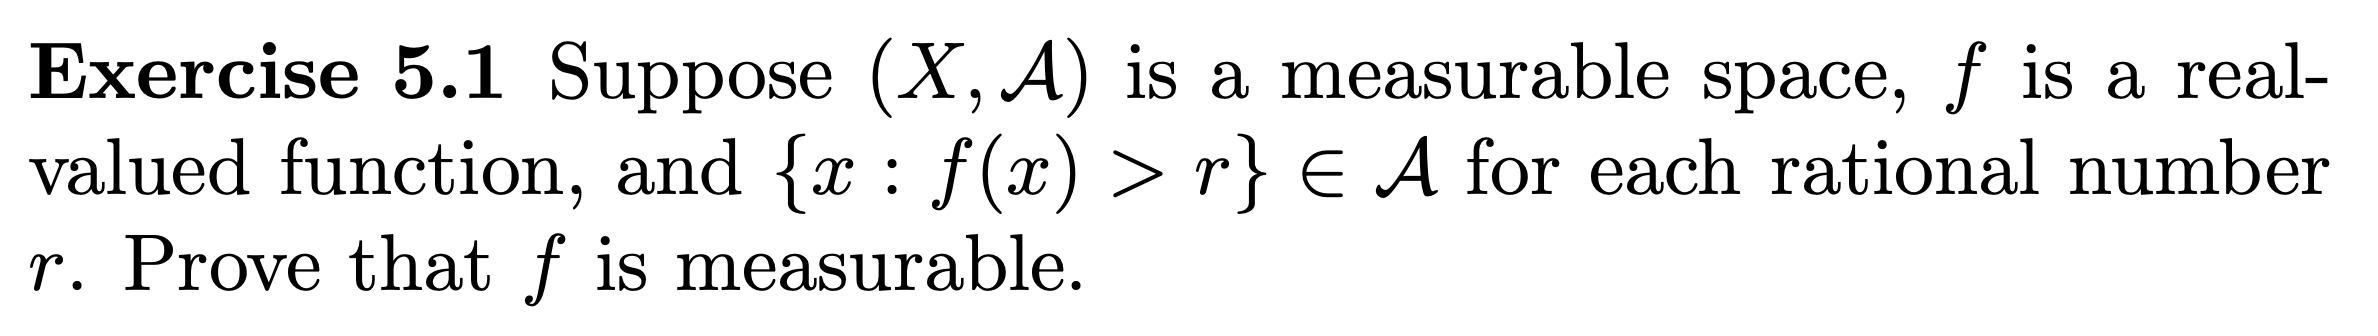
\includegraphics[width=400pt]{img/analysis--berkeley-202a-hw06-ab56.png}
\end{mdframed}

\begin{proof}
  Let $a \in \R$. Define $q_i$ to be the number formed by truncating the decimal expansion of $a$ at the $i$-th
  digit. Then $q_1, q_2, \ldots \in \Q$ is a sequence of rationals with $\lim_{i \to \infty} q_i = a$. Therefore
  \begin{align*}
    \lim_{i \to \infty} \{x ~:~ f(x) > q_i\} = \{x ~:~ f(x) > a\},
  \end{align*}
  and hence
  \begin{align*}
    \{x ~:~ f(x) > a\} = \bigcup_{i=1}^\infty \{x ~:~ f(x) > q_i\}.
  \end{align*}
  Therefore $\{x ~:~ f(x) > a\}$ is a countable union of elements of $\mc A$, for all $a \in \R$. Therefore $f$
  is $\mc A$-measurable.
\end{proof}



\newpage
\begin{mdframed}
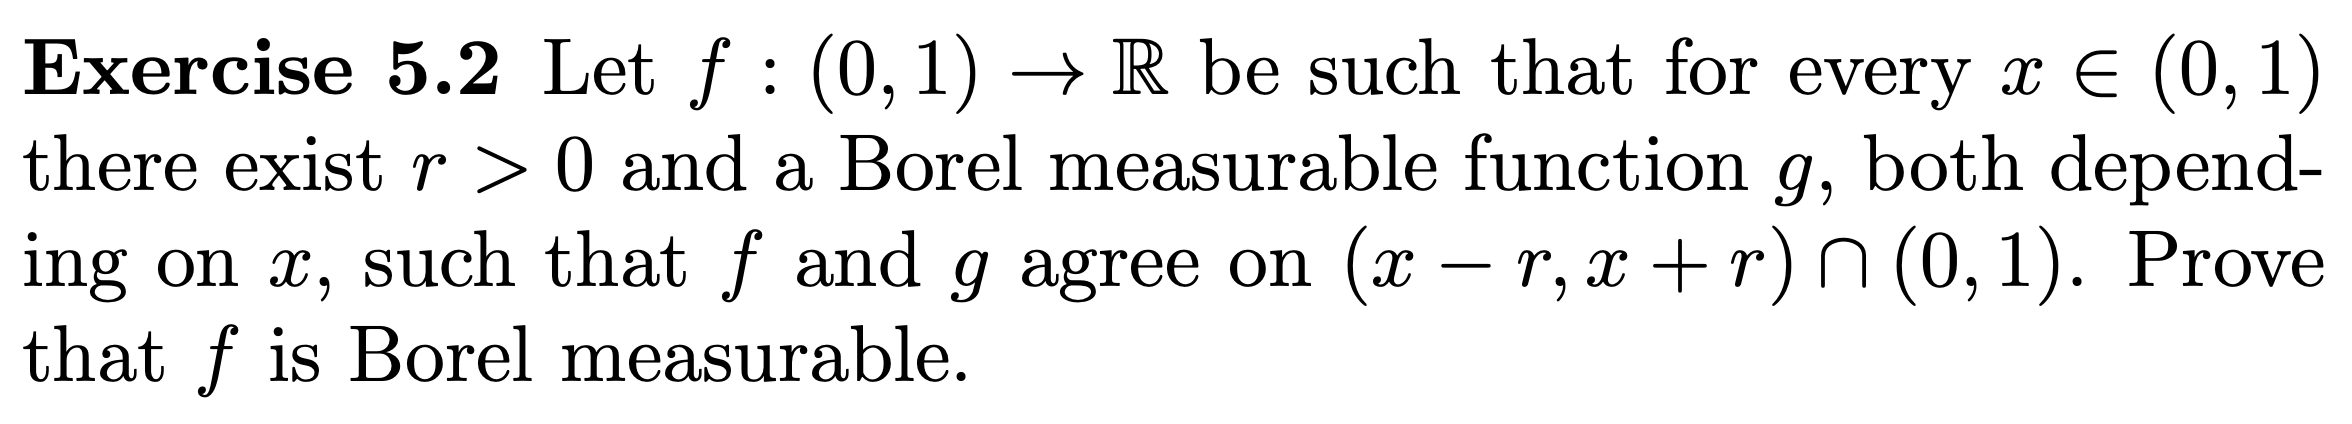
\includegraphics[width=400pt]{img/analysis--berkeley-202a-hw06-927a.png}
\end{mdframed}

\begin{proof}
  Let $\mc A$ be the Borel $\sigma$-algebra on $(0, 1)$ and for every $x \in (0, 1)$ let $r_x > 0$ be such
  that $f$ and $g_x$ agree on $(x - r_x, x + r_x) \cap (0, 1)$, and $g_x$ is Borel-measurable.

  We must show that $\{x ~:~ f(x) > y\} \in \mc A$ for all $y \in \R$.

  Let $y \in \R$ and let $q_1, q_2, \ldots \in \Q \cap (0, 1)$ be an enumeration of the rationals in $(0, 1)$.

  Define $U_{a} := \{x ~:~ g_{a}(x) > y\} \cap (a - r_{a}, a + r_{a})$. Note that $U_a$ is a set of real
  numbers $x$ near $a$ for which we know that $f(x) > y$.

  We claim that $\{x ~:~ f(x) > y\} = \bigcup_{i=1}^\infty U_{q_i} \in \mc A$.

  Let $w = \inf \{r_{q_i} ~:~ i \in \N \}$.

  To prove the forwards inclusion, let $b \in \{x ~:~ f(x) > y\}$, and let $q \in (b - w, b + w) \cap \Q$. Note
  that $b \in (q - r_q, q + r_q)$ and therefore $g_q(b) = f(b) > y$. Therefore $b \in U_q$, proving the
  forwards inclusion.

  To prove the reverse inclusion, let $b \in \bigcup_{i=1}^\infty U_{q_i}$. Then $b \in U_q$ for
  some $q \in \{q_1, q_2, \ldots\}$. Therefore $f(b) > y$.

  Finally, note that $U_a$ is the intersection of two Borel-measurable sets and hence is Borel-measurable.
  Therefore $\bigcup_{i=1}^\infty U_{q_i}$ is Borel-measurable.
\end{proof}



\newpage
\begin{mdframed}
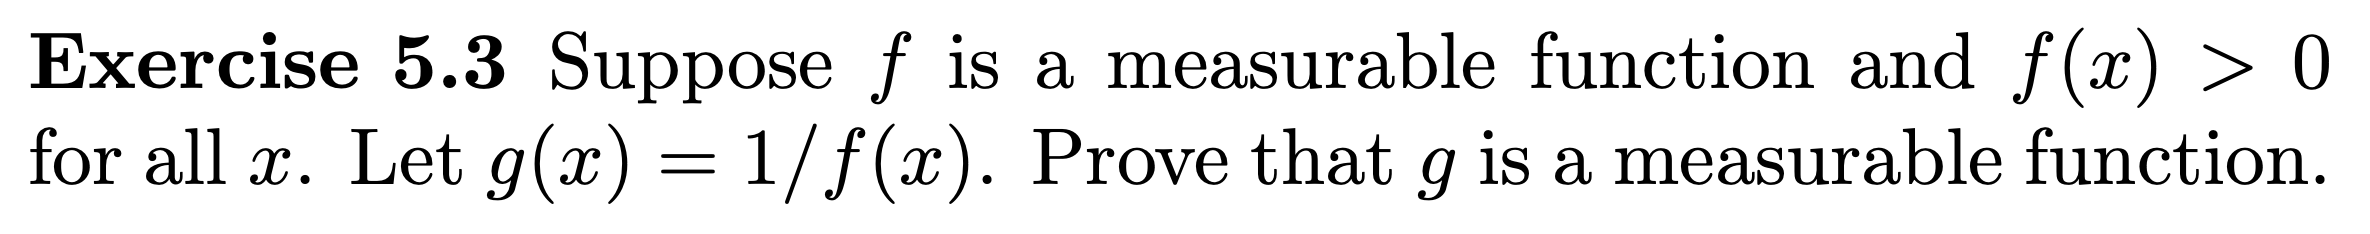
\includegraphics[width=400pt]{img/analysis--berkeley-202a-hw06-b799.png}
\end{mdframed}

\begin{proof}
  Let $f: X \to (0, \infty)$ be a measurable function, and let $g(x) = 1/f(x)$.

  Since $f$ is measurable, there exists a $\sigma$-algebra $\mc A$ such that $f^{-1}((y, \infty)) \in \mc A$
  for all $y > 0$.

  Let $h(x) = 1/x$. Then $g = h \circ f$.

  Fix $y \in (0, \infty)$ and let $U = h^{-1}((y, \infty)) \subseteq (0, \infty)$. Since $h$ is
  continuous, $U$ is open.

  We want to show that $g^{-1}((y, \infty)) \in \mc A$. We have
  \begin{align*}
    g^{-1}((y, \infty)) = f^{-1}(h^{-1}((y, \infty))) = f^{-1}(U).
  \end{align*}
  So what we want to show is that $f^{-1}(U) \in \mc A$, where $U \subseteq (0, \infty)$ is open.

  Write $U = \bigcup_{i=1}^\infty (a_i, b_i)$ where $(a_1, b_1), (a_2, b_2), \ldots \subseteq (0, \infty)$ is a
  countable pairwise disjoint collection of open intervals.

  Note that $f^{-1}(U) = \bigcup_{i=1}^\infty f^{-1}((a_i, b_i))$.

  Note also that $(a, b) = (a, \infty) \setminus (b, \infty)$ and therefore
  that $f^{-1}((a, b)) = f^{-1}((a, \infty)) \setminus f^{-1}((b, \infty))$.

  Thus we have
  \begin{align*}
    f^{-1}(U)
    &= \bigcup_{i=1}^\infty \Big(f^{-1}((a, \infty)) \setminus f^{-1}((b, \infty))\Big) \\
    &= \bigcup_{i=1}^\infty \Big(f^{-1}((a, \infty)) \cap \big(f^{-1}((b, \infty))\big)^c\Big) \\
    &\in \mc A,
  \end{align*}
  since this is a countable union of intersections of two sets that are both in $\mc A$ (one by definition, and
  one as the complement of a set that is in $\mc A$ by definition).
\end{proof}


\newpage
\begin{mdframed}
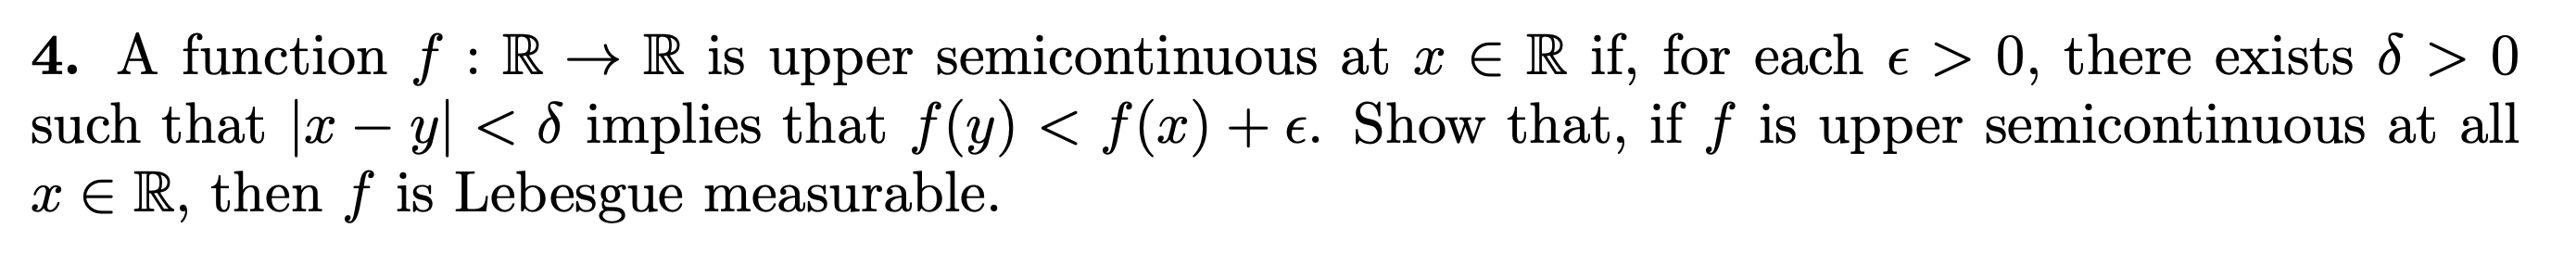
\includegraphics[width=400pt]{img/analysis--berkeley-202a-hw06-90b1.png}
\end{mdframed}


\begin{proof}
  It suffices to show that $f^{-1}\((-\infty, y)\)$ is open for all $y \in \R$, since
  then $f^{-1}\((-\infty, y)\)$ is Borel-measurable, and therefore Lebesgue-measurable.

  % We know that there is a theorem concerning continuous functions on metric/topological spaces: $f:\R \to \R$
  % is
  % continuous if and only
  % if $f^{-1}(U)$ is open for every open subset $U \subseteq \R$.

  % We want to prove the reverse direction of this, but assuming upper semicontinuity only. In other words, we
  % want to prove that (upper semicontinuity) implies (preimage of $(-\infty, q)$ is open) for all $q \in \R$.

  % We follow the proof of the standard theorem (see Kevin McGerty's Oxford A2 Metric Spaces notes) but
  % substituting upper semicontinuity.

  So, fix $y \in \R$ and let $a \in f^{-1}\((-\infty, y)\)$. It suffices to show that $f^{-1}\((-\infty, y)\)$
  includes a neighborhood of $a$, since then it contains a neighborhood of all its points and therefore is
  open as required.

  Since $f$ is upper semicontinuous there exists $\eps > 0$ and $\delta > 0$ such
  that $(a - \delta, a + \delta) \subset f^{-1}\((-\infty, f(a) + \eps)\)$.

  Note that $f(a) \in (-\infty, y)$.
  Therefore $(a - \delta, a + \delta) \subset f^{-1}\((-\infty, y + \eps)\)$.

  Since $\eps$ is arbitrary we have that $(a - \delta, a + \delta) \subseteq f^{-1}\((-\infty, y)\)$, and
  therefore that $f^{-1}\((-\infty, y)\)$ includes a neighborhood of $a$, as required.
\end{proof}

\newpage
\begin{mdframed}
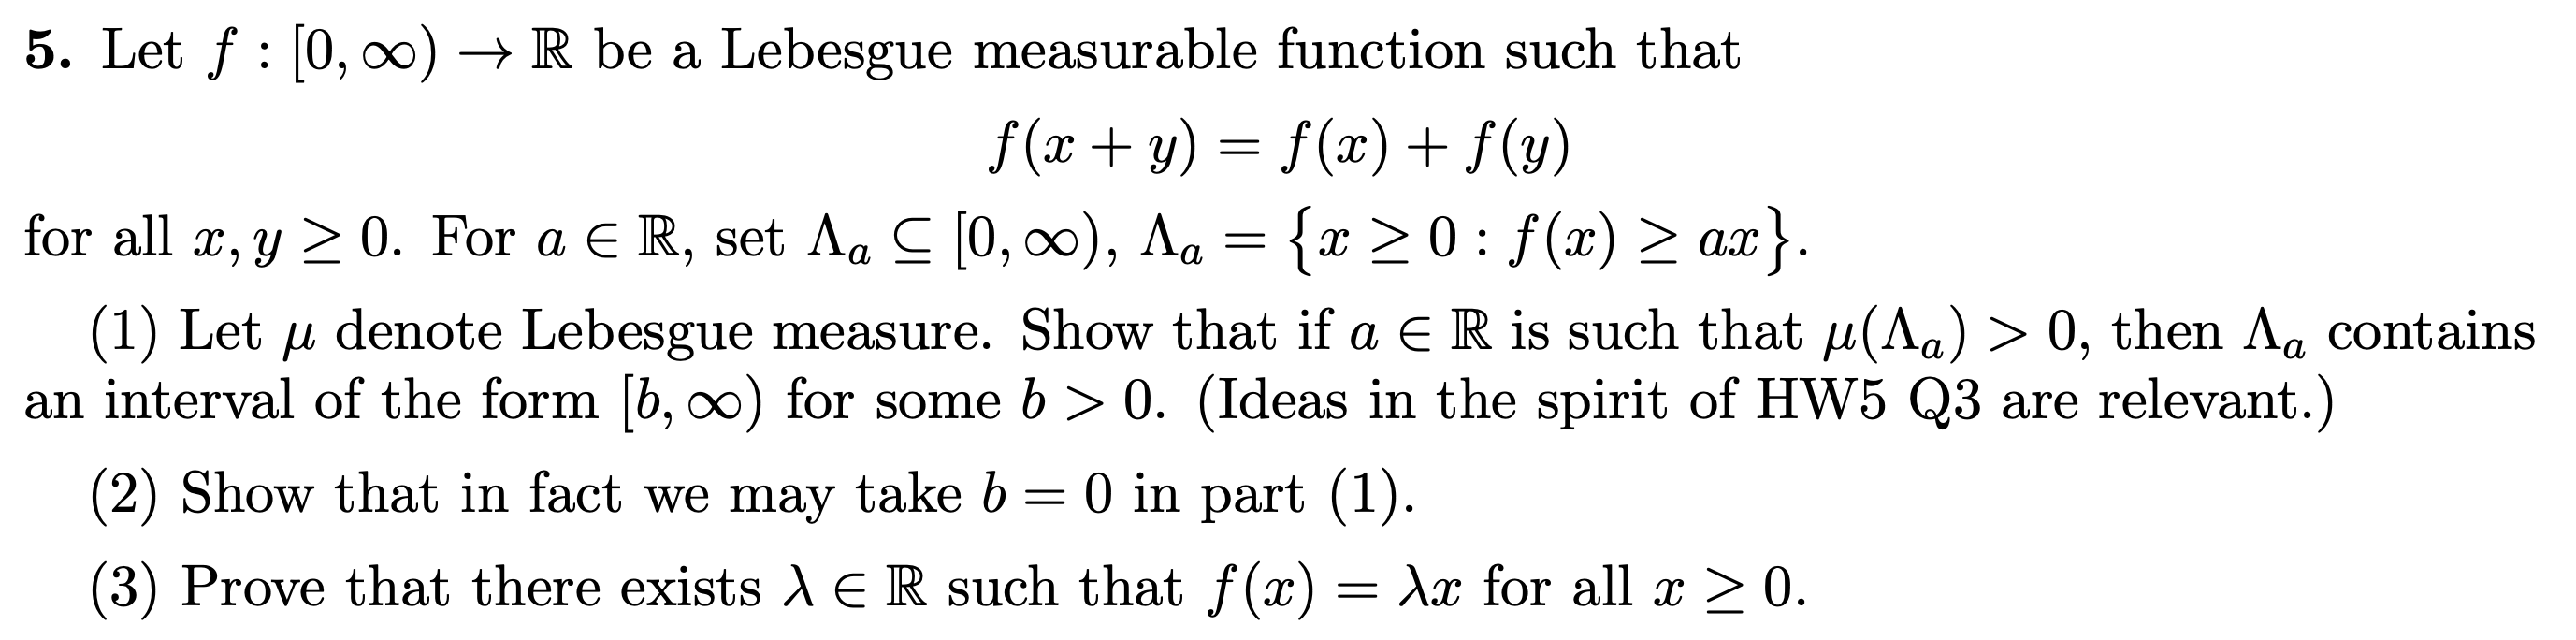
\includegraphics[width=400pt]{img/analysis--berkeley-202a-hw06-7769.png}
\end{mdframed}

Note that $f(0) = 0$, since $f(0) = f(0 + 0) = 2f(0)$, of which the only solution is $f(0) = 0$.

For $a \in \R$ define $g_a(x) := f(x) - ax$ so that $\Lambda_a = \{x \geq 0 ~:~ g_a(x) \geq 0\}$.

Note that $g_a$ is measurable for all $a \in \R$, and therefore $\Lambda_a$ is Lebesgue measurable for
all $a \in \R$. To see this, for $a \in \R$ define $h_a(x) = -ax$ so that $g_a = f + h_a$. Then $h_a$ is
clearly Lebesgue measurable for all $a \in \R$, and therefore so also is $g_a(x)$ (by Bass proposition 5.7
which states that a function produced via elementary operations on measurable functions is measurable).

\begin{align*}
  f(4 - 3) = f(4) + f(-y)
\end{align*}


\begin{enumerate}
\item
  \begin{claim*}
    If $a \in \R$ is such that $\mu(\Lambda_a) > 0$ then $\Lambda_a$ includes an interval $[b, \infty)$ for some $b > 0$.
  \end{claim*}

  \begin{proof}
    Let $\eps > 0$. Since $\Lambda_a$ is Lebesgue measurable there exists an open set $G \supseteq \Lambda_a$
    such that $\mu(G \setminus \Lambda_a) < \eps/2$ and a closed set $F \subseteq \Lambda_a$ such
    that $\mu(\Lambda_a \setminus F) < \eps/2$. Thus we have $F \subseteq \Lambda_a \subseteq G$
    with $\mu(G) - \mu(F) < \eps$.

    We will show that for all $a \in \R$ there exists $b > 0$ such that $g_a(x) \geq 0$ for $x \in [b, \infty)$.

    We must use: additivity of $f$, positive measure of $\{x ~:~ g_a(x) \geq 0\}$.

    \begin{align*}
      g_a\Big(\sum_{x \in \Lambda_a} x\Big) = \sum_{x \in \Lambda_a} g_a(x) \geq 0.
    \end{align*}

    Note that for all $n \in \N$ we have $f(nx) = f(x + x + \cdots + x) = nf(x)$. Therefore
    \begin{align*}
      g_a(nx)
      &= f(nx) - anx \\
      &= n(f(x) - ax) \\
      &= ng_a(x).
    \end{align*}
    \begin{align*}
      g_a(x + x')
      &= f(x + x') - a(x + x') \\
      &= g_{a}(x) + g_{a}(x').
    \end{align*}
    Since $\mu(\Lambda_a) > 0$ there exist $x$ and $x'$ such that $g_a(x) \geq 0$ and $g_a(x') \geq 0$
    and $x \neq x'$.

    Therefore $g_a(x + x') \geq 0$.

    So what we need to do is show that some interval $[b, \infty)$ is ``spanned​'' by $x, x'$ values in $\Lambda_a$.

    \begin{align*}
      f(x + x)
      &= f(x) + f(x) \\
      &= 2f(x)
    \end{align*}


  \end{proof}

\item
  \begin{claim*}
    If $a \in \R$ is such that $\mu(\Lambda_a) > 0$ then $\Lambda_a$ includes an interval $[0, \infty)$.
  \end{claim*}

\item
  \begin{claim*}
    There exists $\lambda \in \R$ such that $f(x) = \lambda x$ for all $x \geq 0$.
  \end{claim*}


\end{enumerate}


\newpage
\begin{mdframed}
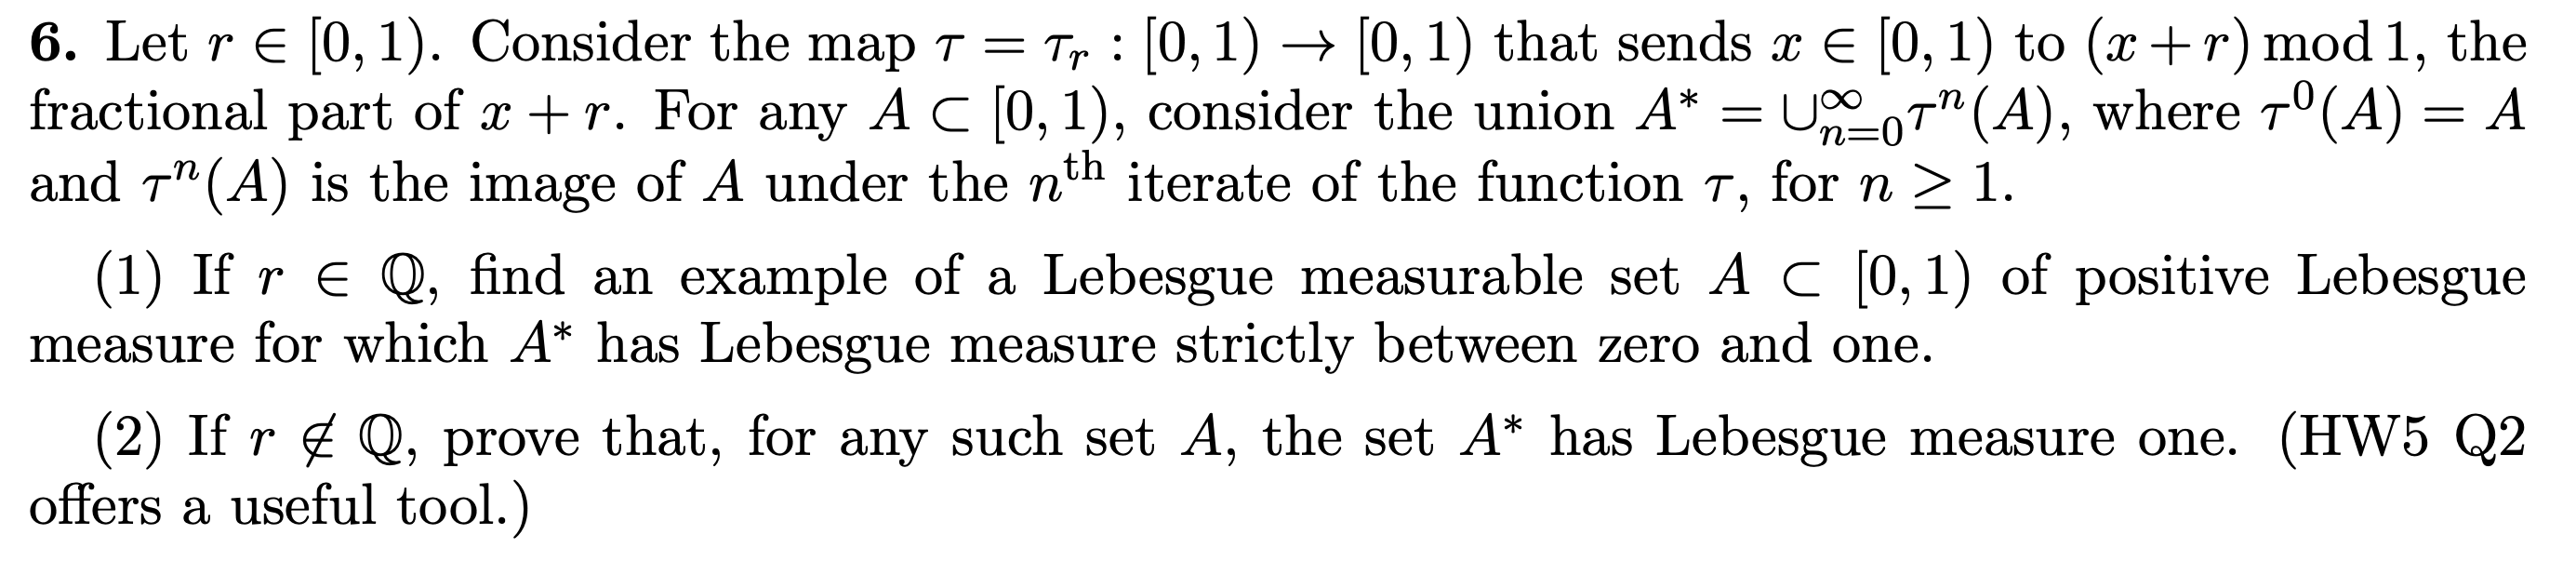
\includegraphics[width=400pt]{img/analysis--berkeley-202a-hw06-9bc5.png}
\end{mdframed}